\documentclass{article}

\usepackage[brazil]{babel}    % português do Brasil
\usepackage[utf8]{inputenc}   % acentos no UTF-8
\usepackage[T1]{fontenc}      % para hifenização correta
\usepackage[a4paper,margin=2.5cm]{geometry}
\usepackage{graphicx}
\usepackage{float}
\usepackage{booktabs}
\usepackage{multirow}
\usepackage{tabularx}
\usepackage{placeins}
\usepackage{xcolor}
\usepackage{xltabular}
\usepackage{subcaption}
\usepackage{caption}
\usepackage{amsmath}
\usepackage[toc,page]{appendix}
\usepackage[style=authoryear, backend=biber]{biblatex}
\addbibresource{referencias_syntaxshap.bib}
\usepackage{hyperref}
\usepackage[most]{tcolorbox}

\renewcommand{\arraystretch}{1.5}
\captionsetup{font=small}

\setlength{\parskip}{0.5em}

\begin{document}

\newpage
\subsection{SyntaxSHAP}

Foi realizada uma busca por trabalhos que citam o SyntaxSHAP \parencite{amara2024syntaxshap} desde sua publicação, com o objetivo de mapear como o método tem sido utilizado pela comunidade, o que a literatura recente diz sobre suas características e limitações, e qual a relação entre os artigos citantes e o método original. Essa investigação busca reunir subsídios para a decisão de utilizar o SyntaxSHAP como técnica de XAI no experimento desta pesquisa, avaliando se o método permanece relevante e se já existe algum uso prévio relacionado ao contexto de Prompt Injection.

\paragraph{Resultados da Busca} Foram encontrados \textbf{14 artigos} que citam o SyntaxSHAP na plataforma Semantic Scholar. Nenhum desses trabalhos foi publicado na ACL Anthology; todos estão disponíveis como preprints no arXiv, concentrados majoritariamente entre 2025 e 2026 (Figura \ref{fig:citacoes-syntaxshap}).

\begin{figure}[H]
    \centering
    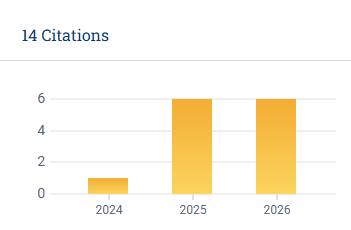
\includegraphics[width=0.8\linewidth]{figs/citacoes_por_ano_syntaxshap.png}
    \caption{Citações do SyntaxSHAP por ano no Semantic Scholar.}
    \label{fig:citacoes-syntaxshap}
\end{figure}

Na Tabela \ref{tab:syntaxshap-citacoes} estão presentes os artigos mais relevantes identificados nessa busca, isto é, aqueles que discutem o SyntaxSHAP com maior profundidade em suas seções de trabalhos relacionados.

\begin{table}[H]
    \centering
    \small
    \caption{Artigos relevantes que citam o SyntaxSHAP}
    \begin{tabularx}{\linewidth}{p{6cm} X}
        \toprule
        \textbf{Artigo} & \textbf{Detalhes} \\
        \midrule

        \textcite{li2026moeflowmatching} & Cita o SyntaxSHAP apenas na lista de referências, sem qualquer menção, descrição ou uso no corpo do artigo. A relação é puramente temática (ambos pertencem à área de PLN), sem vínculo metodológico. \\

        \textcite{ciaperoni2026comparing} & Cita o SyntaxSHAP de passagem, como exemplo de método de XAI tradicional de atribuição de \textit{features} do tipo ``single-checkpoint'' (ao lado do LIME), sem aplicá-lo experimentalmente. Argumenta que métodos desse tipo são insuficientes para explicar mudanças comportamentais entre versões de um modelo, servindo de contraponto à proposta do artigo (XAI comparativo). \\

        \textcite{mohammadi2025tokenreplacement} & Menciona o SyntaxSHAP na seção de trabalhos relacionados, descrevendo-o como uma extensão do SHAP que atribui importância a constituintes sintáticos em vez de tokens individuais. Optou por usar SHAP e LIME padrão por serem \textit{model-agnostic}, deixando o SyntaxSHAP citado apenas como alternativa não escolhida. \\

        \textcite{amara2025conceptlevel} & Escrito pelos próprios autores do SyntaxSHAP, propõe o ConceptX como evolução do método. Justifica a exclusão do SyntaxSHAP das comparações experimentais afirmando que ele é otimizado para a log-probabilidade das saídas do modelo, sendo escalável apenas para tarefas de geração de token único (ex.: classificação), e inadequado para geração de resposta completa. \\

        \textcite{yan2025explainablemapper} & Cita o SyntaxSHAP na revisão de métodos de perturbação de texto, descrevendo-o como uma técnica que remove palavras preservando a coerência gramatical, em contraste com perturbações aleatórias. Serve de base conceitual para os \textit{Verification Agents} propostos, que também usam substituições preservando o sentido do texto. \\

        \bottomrule
    \end{tabularx}
    \label{tab:syntaxshap-citacoes}
\end{table}

\paragraph{Principais Achados} Embora vários artigos recentes proponham novos métodos de XAI e citem o SyntaxSHAP, nenhum deles o implementa ou o utiliza como \textit{baseline} em comparações experimentais. Chama atenção o fato de os próprios autores do SyntaxSHAP terem desenvolvido uma nova técnica, o ConceptX \parencite{amara2025conceptlevel}, alegando que o método original não é adequado para tarefas de geração de resposta completa — o que, por outro lado, reforça sua adequação para tarefas de token único, como classificação, que é justamente o cenário de interesse deste trabalho (a detecção de Prompt Injection pelo PromptGuard). De maneira geral, o SyntaxSHAP é citado como um dos métodos de referência para técnicas de XAI baseadas em perturbação que respeitam a estrutura gramatical do texto, mas os artigos mais recentes tendem a citá-lo apenas como trabalho anterior, sem incorporá-lo em comparações, priorizando a proposta de novas técnicas em vez do aprimoramento ou aplicação das já existentes.

\subsubsection{Justificativa de uso}

Diante do exposto, opta-se por utilizar o SyntaxSHAP como técnica de XAI no experimento desta pesquisa. O método é um dos pioneiros em explicabilidade baseada em perturbação com coerência sintática, sendo bem fundamentado por ter sido publicado na ACL Anthology \parencite{amara2024syntaxshap}. Apesar de citado por trabalhos recentes, o método não foi efetivamente reaproveitado ou expandido por esses artigos, e não há, até o momento, nenhuma aplicação do SyntaxSHAP em contextos de Prompt Injection — o que caracteriza uma lacuna de pesquisa a ser explorada. Assim, este trabalho se propõe a dar um primeiro passo nessa direção, avaliando a performance de métodos de XAI, começando pelo SyntaxSHAP, em benchmarks de Prompt Injection.

\printbibliography

\end{document}
